\documentclass[11pt]{article}
    %	options include 12pt or 11pt or 10pt
    %	classes include article, report, book, letter, thesis

    \usepackage{amsmath}
    \usepackage{array}
    \setlength\extrarowheight{2pt}
    \usepackage{graphicx}
    \usepackage{epstopdf}
    \usepackage{graphics}
    \graphicspath{ {/home/shanedrafahl/coms331/hw0} }
    
    \title{HW3}
    \author{Shane Drafahl}
    \date{26 September,2017}

    \begin{document}
    \maketitle

    1. (a) 

    \begin{figure}[!htb]
        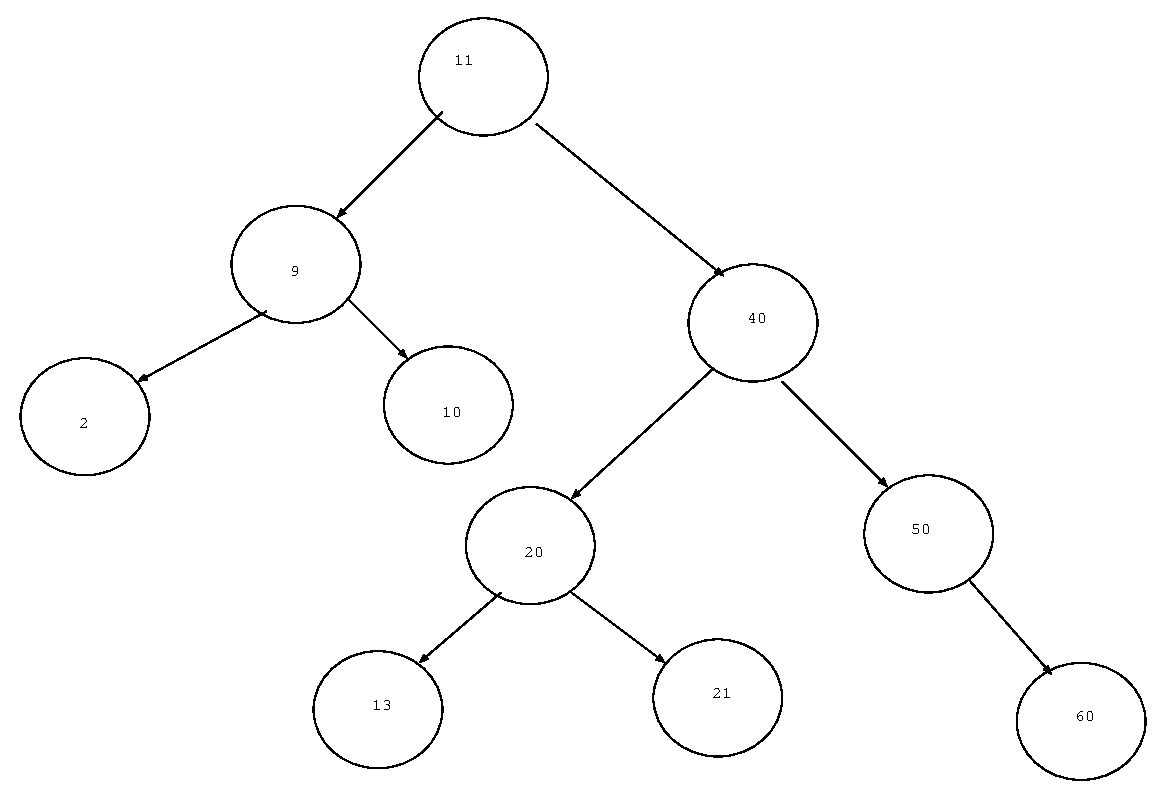
\includegraphics[scale=.7]{./unbalanced.eps}
    \end{figure}
    
    $ \newline \newline $

    (b).
        Every node in this tree follows the requirements to be an AVL tree. Every node
        has a difference of height for it children that is either -1,0,1.

        $ \newline \newline $

    (c).
        $ (2x + 3) $ mod $ 5 \leq 4 $ so we can assume the hashset only has a size of 4.
        
        $ \newline \newline $
        \begin{figure}[!htb]
            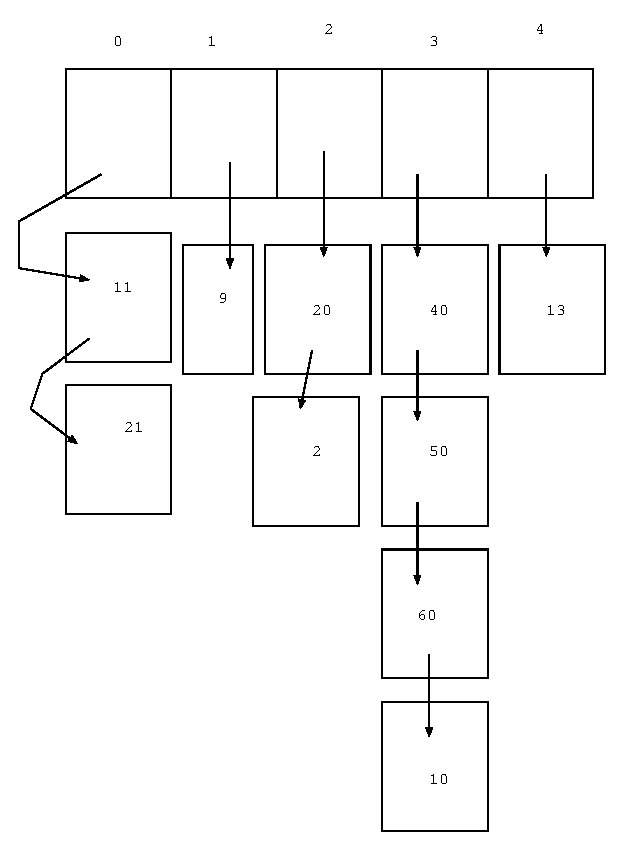
\includegraphics[scale=.7]{./hash.eps}
        \end{figure}
        
        $ \newline \newline $

        2. Consider that binary tree T is a perfectly balanced tree so each node must
        have 2 children or 0 children. The tree has $ n = 2^{ \ell } - 1 $ 
        distinct integers so the tree must have n nodes.
        
        $ \newline $

        Lemma $ n = 2^{h + 1} - 1 $ where h is the height of the binary tree.

        $ \newline $

        Basis: Suppose a tree $ T^{'} $ has only a single root node so h = 0.
        $ 1 = 2^{1} - 1 $.

        $ \newline $

        Inductive Hypothesis: 
        Suppose that $ n = 2^{h + 1} - 1 $ is true for tree $T_{1}$, $T_{2}$.

        $ \newline $

        Recursion:

        Using structural induction for $ T_{1} $, $ T_{2} $
        returns the number of node for each tree $ n = 2^{h + 1} - 1 $ where
        h is the height for either tree. Both trees need to have the same 
        height or else the new binary tree might not be perfectly balanced .
        If we combine $ T_{1} $ and $ T_{2} $ and for order it to be a perfectly balanced tree
        we will add a single node N that will be the new root node that is a parent
        with the roots from $ T_{1} $ and $ T_{2} $. The height of the new tree 1 + h 
        the number of nodes. The number of nodes in the new tree will be 
        $ 2^{h + 1} - 1 $ + $ 2^{h + 1} - 1 $ + 1 or it can be reduced to 
        $ 2^{h + 2} - 2 + 1$ ... $ n = 2^{h + 2} - 1 $. Since $ 1 + h = h^{'}$
        the new tree will have $ 2^{h^{'} + 1} - 1 $ nodes. So therefore for all 
        perfectly balanced trees there are $ 2^{h + 1} - 1 $ nodes for its height h.
        QED

        $ \newline $

        $ n = 2^{ \ell } - 1 $ is the number of nodes in the tree so therefore 
        $ \ell $ = h + 1 where h is the height of the tree. 
        
        $ \newline $

        The algorithm is 

        \begin{verbatim}
            // T is a tree
            // T.R is the root node
            // T.R.L is the left child of the root
            // T.R.R is the right child of the root

            getElementSmallerThan(T) {
                return T.R.R
            }

        \end{verbatim}

        $ \newline $

        This algorithm is obviously O(1) this algorithm is correct because 
        by the lemma there are $ 2^{h + 1} - 1 $ nodes in the tree and we want a 
        value that is smaller than $ 2^{h - 1} - 1 $ nodes. If there are $ a $ 
        nodes in the tree then we need to find the node smaller than 
        $ \frac{a + 1}{4} - 1 $ nodes. Notice that $ \frac{a + 1}{4} - 1 $
        equals the number of nodes in the subtree of the right child of the 
        right child of the root node. This makes sense because it should be
        about a fourth of the nodes it needs to be smaller than. For a tree
        of three nodes the right child has no children so $ \frac{3 + 1}{4} - 1 $ = 0
        so in that case the right child of the root would be the largest
        value in the tree being smaller than 0 values in the tree. For larger
        trees almost a quarter of the entire tree is the subtree of the right child of the
        right child of the root. Meaning that the right child of the root is smaller than
        $ 2^{ \ell - 2 } - 1 $ or $ n = 2^{ h - 1 } - 1 $ elements in the tree. QED
        
        $ \newline \newline $

        (b) We start with a tree that looks like
        \begin{figure}[!htb]
            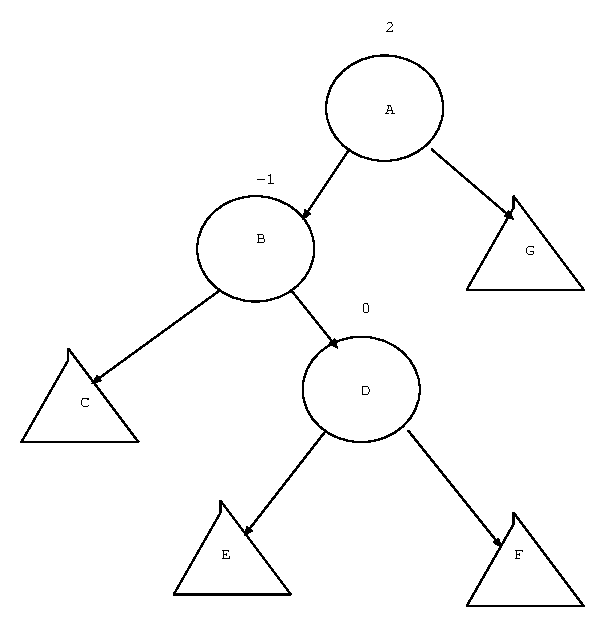
\includegraphics[scale=.7]{./preBalanced.eps}
        \end{figure}


    \end{document}
